\usepackage[left = 2.75cm, top = 1cm]{geometry}
%\usepackage[utf8]{inputenc}
%\usepackage[utf8]{inputenc}
%\usepackage[utf8]{inputenc}
\usepackage[T1]{fontenc}
\usepackage[english]{babel}
\usepackage{amsfonts}
\usepackage{ifthen}
\usepackage{mdframed}
%\usepackage{amssymb}
%\usepackage[margin=0.5cm, paper width=100cm, paper height=100cm]{geometry}
\usepackage{amsmath}
\usepackage{amsthm}
\usepackage{verbatim}
\usepackage{array}
\usepackage{booktabs}
%\usepackage[sc]{mathpazo}
\usepackage{multirow}
\usepackage[table]{xcolor}
\usepackage{datetime}

\renewcommand{\familydefault}{\sfdefault}

\setlength{\heavyrulewidth}{1.5pt}
\setlength{\abovetopsep}{4pt}
\renewcommand{\qedsymbol}{$\blacksquare$}
\newcommand\numberthis{\addtocounter{equation}{1}\tag{\theequation}}
\setlength{\marginparwidth}{3.5cm}
\usepackage{graphicx}
\usepackage[square%round
, colon]{natbib}
\setcitestyle{aysep={},yysep={;}}
\usepackage{capt-of}
\usepackage{tikz}
\usepgflibrary{arrows}
\usetikzlibrary{shapes}
\usetikzlibrary{calc}
\usetikzlibrary{decorations}
\usetikzlibrary{decorations.pathmorphing}
\usetikzlibrary{decorations.shapes}
\usetikzlibrary{decorations.pathreplacing}
\usetikzlibrary{intersections}
%\frenchspacing
\title{Órarend}
\author{Attila Molnár}

\newcommand{\oda}[5][]{\begin{tikzpicture}[remember picture,overlay]
\node[#1] at ([xshift=#3 cm, yshift=#4 cm]current page.#2){#5};
\end{tikzpicture}}



\newcommand{\ora}[3]{
%1 Nap
%2 Óra
%3 Beírandó termek
	\pgfmathtruncatemacro{\egysucc}{#1+1}
%	\filldraw[draw=black, ultra thick](BFS#1-#2) rectangle (JFS\egysucc-#2);
	\node[inner sep=1mm, anchor=north east, scale=1] at (BFS#1-#2) {\scalebox{2}{\begin{minipage}{2 cm}#3\end{minipage}}};
} % end of \newcommand{ora}

\newcommand{\skeleton}{
\begin{tikzpicture}[remember picture,overlay]
		\pgfmathsetmacro\opn{6}
		\pgfmathsetmacro\szelesseg{4.6} 
		\pgfmathsetmacro\magassag{3}
		\pgfmathsetmacro\cimkeszel{0}
		\pgfmathsetmacro\cimkemag{1}

\coordinate (Csigolya0) at (0,0);
\coordinate[xshift=-\cimkeszel cm] (evcStart0) at (Csigolya0);
\pgfmathsetmacro{\teljesszelesseg}{\cimkeszel+5*\szelesseg }
\coordinate[xshift= \teljesszelesseg cm] (evcEnd0) at (Csigolya0);
\draw[ultra thick] (evcStart0)--(evcEnd0);
	
\foreach \i in {1,...,\opn}
{
	\pgfmathtruncatemacro{\preci}{\i-1}
	\coordinate (Csigolya\i) at ([yshift=-\magassag cm]Csigolya\preci);
	\coordinate (evcStart\i) at ([yshift=-\magassag cm]evcStart\preci);
	\coordinate (evcEnd\i)   at ([yshift=-\magassag cm]evcEnd\preci);
	\path (Csigolya\i)--(Csigolya\preci) 
		node[anchor=base, inner sep=2mm, midway, left]{\scalebox{4}{\i.}};
%	\path (evcEnd\i)--(evcEnd\preci) 
%		node[anchor=base, inner sep=2mm, midway, right, xshift=-\cimkeszel cm]{\scalebox{4}{\i.}};
}%end of \foreach \i/\tanar in \tanarlista



%Bal felső és jobb felső sarkok elnevezése
\foreach \ora in {1,...,\opn}
{	\pgfmathtruncatemacro{\predora}{\ora-1}
	\foreach\nap in {1,...,6}
	{	
		\coordinate[xshift=\nap*\szelesseg cm] (BFS\nap-\ora) at (Csigolya\predora);
		\coordinate[xshift=\szelesseg cm] (JFS\nap-\ora) at (BFS\nap-\ora);
	}%end of \foreach \nap
}%end of \foreach \ora

% FÜGGŐLEGES VONALAK. Két ciklus egymásban. Az egyik a napokat pakolja, a másik azon belül az órákat.
% plusz utána a lezárása.
\foreach \napszam/\napnev in {1/h{\' e}tf{\H o}, 2/kedd, 3/szerda, 4/cs{\" u}t{\" o}rt{\" o}k, 5/p{\' e}ntek}
	{
		\pgfmathsetmacro{\honnan}{(\napszam-1)*\szelesseg}
		\node[anchor=south] at (\honnan + 0.5*\szelesseg,.25*\cimkemag){\scalebox{2.3}{\textsc{\napnev}}};
		\draw[ultra thick] (\honnan, \cimkemag) 
									 -- (\honnan, -\opn*\magassag);
	}
		\pgfmathsetmacro{\honnan}{(6-1)*\szelesseg}
		\draw[ultra thick] (\honnan, \cimkemag) 
									 -- (\honnan, -\opn*\magassag);
	

\foreach \i in {1,...,\opn} {\draw[ultra thick] (evcStart\i)--(evcEnd\i);}


\end{tikzpicture}
\thispagestyle{empty}}%end of skeleton

\newcommand{\orarend}{
	\begin{tikzpicture}[remember picture, overlay]
		
\ora{1}{1}{Ol.t R. K.ea Tt.s. }
\ora{1}{2}{Ol.t Tt.s. }
\ora{1}{3}{M. Ol.t II.43 R. Tt.s. }
\ora{1}{4}{Ol.t Tt.s. }
\ora{1}{5}{Ol.t Tt.s. }
\ora{1}{6}{F.18 Ol.t II.41 Tt.s. }
\ora{2}{1}{É. Ol.t II.41 Tt.s. }
\ora{2}{2}{Ol.t Tt.s. }
\ora{2}{3}{L. Ol.t Fiz. Tt.s. }
\ora{2}{4}{F.12 Ol.t R. Tt.s. }
\ora{2}{5}{Ol.t Tt.s. }
\ora{2}{6}{F.18 I.30 I.33 I.34 M. Ol.t II.40 II.42 Tt.s. }
\ora{3}{1}{É. Ol.t II.41 II.44 II.51 Tt.s. }
\ora{3}{2}{Ol.t Fiz. Tt.s. }
\ora{3}{3}{A.1 Ol.t II.41 Tt.s. }
\ora{3}{4}{N. F.8 F.9 F.11 F.17 Fr. Sp. Ol.t Tt.s. }
\ora{3}{5}{Ol.t II.44 Tt.s. }
\ora{3}{6}{Ol.t Tt.s. }
\ora{4}{1}{Fiz. Tt.s. }
\ora{4}{2}{Ol.t Tt.s. }
\ora{4}{3}{Ol.t R. Tt.s. }
\ora{4}{4}{Ol.t II.50 Tt.s. }
\ora{4}{5}{Ol.t II.40 Tt.s. }
\ora{4}{6}{N. É. F.10 Ol.t R. Tt.s. }
\ora{5}{1}{Ol.t II.41 II.43 Tt.s. }
\ora{5}{2}{F.9 F.11 Ol.t R. Tt.s. }
\ora{5}{3}{Ol.t R. Fiz. Tt.s. }
\ora{5}{4}{F.8 Ol.t II.51 Tt.s. }
\ora{5}{5}{É. Sp. Ol.t II.51 R. Tt.s. }
\ora{5}{6}{É. F.9 F.10 Fr. Sp. Ol.t II.48 Tt.s. }

	\end{tikzpicture}
}%endof \orarend
